% 固定来源PDF印刷页52第10题正方体及E_1、F_1位置的矢量示意重绘。
% 深度方向使用斜投影；比例仅作示意，点分段比例按题面标注。
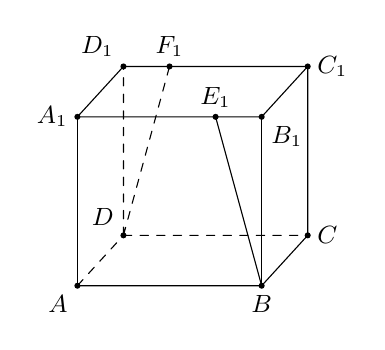
\begin{tikzpicture}[x=.78cm,y=.78cm,font=\small,line cap=round,line join=round]
  \coordinate (A) at (0,0);
  \coordinate (B) at (3,0);
  \coordinate (C) at (3.75,.82);
  \coordinate (D) at (.75,.82);
  \coordinate (Aone) at (0,2.75);
  \coordinate (Bone) at (3,2.75);
  \coordinate (Cone) at (3.75,3.57);
  \coordinate (Done) at (.75,3.57);
  \coordinate (Eone) at (2.25,2.75);
  \coordinate (Fone) at (1.5,3.57);

  % Visible and hidden cube edges follow the source perspective drawing.
  \draw (A)--(B)--(C)--(Cone)--(Bone)--(Aone)--(Done)--(Cone);
  \draw (A)--(Aone) (B)--(Bone) (Done)--(Fone);
  \draw[dashed] (A)--(D) (D)--(C) (D)--(Done) (D)--(Fone);
  % The two lines whose angle is asked for.
  \draw (B)--(Eone);

  \fill (A) circle (1.1pt) (B) circle (1.1pt) (C) circle (1.1pt) (D) circle (1.1pt)
        (Aone) circle (1.1pt) (Bone) circle (1.1pt) (Cone) circle (1.1pt) (Done) circle (1.1pt)
        (Eone) circle (1.1pt) (Fone) circle (1.1pt);
  \node[below left] at (A) {$A$};
  \node[below] at (B) {$B$};
  \node[right] at (C) {$C$};
  \node[above left] at (D) {$D$};
  \node[left] at (Aone) {$A_1$};
  \node[below right] at (Bone) {$B_1$};
  \node[right] at (Cone) {$C_1$};
  \node[above left] at (Done) {$D_1$};
  \node[above] at (Eone) {$E_1$};
  \node[above] at (Fone) {$F_1$};
\end{tikzpicture}
